\documentclass[tikz,border=10pt]{standalone}
\usepackage{tikz}
\usepackage{amsmath,amssymb}
\usetikzlibrary{shapes,arrows.meta,positioning,calc,fit,backgrounds,decorations.pathreplacing}

\begin{document}
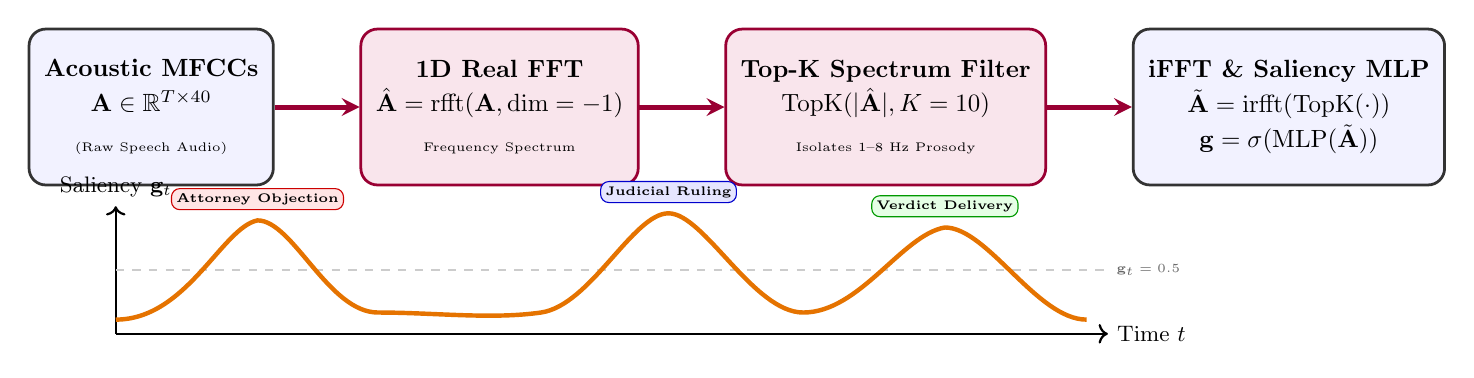
\begin{tikzpicture}[
    scale=0.9,
    every node/.style={transform shape},
    box/.style={draw=black!80, rectangle, rounded corners=6pt, fill=blue!5, line width=1.0pt, align=center, inner sep=6pt},
    proc/.style={draw=purple!80!black, rectangle, rounded corners=6pt, fill=purple!10, line width=1.0pt, align=center, inner sep=6pt},
    gate/.style={draw=orange!80!black, circle, fill=orange!20, line width=1.0pt, inner sep=2pt, font=\small\bfseries}
]

    % Stage 1: Input MFCC Acoustic Stream
    \node[box, minimum width=3.2cm, minimum height=2.2cm] (mfcc) at (0,0) {
        \textbf{Acoustic MFCCs}\\[2pt]
        $\mathbf{A} \in \mathbb{R}^{T \times 40}$\\[4pt]
        \tiny (Raw Speech Audio)
    };

    % Stage 2: RFFT Frequency Decomposition
    \node[proc, minimum width=3.4cm, minimum height=2.2cm, right=1.2cm of mfcc] (rfft) {
        \textbf{1D Real FFT}\\[2pt]
        $\hat{\mathbf{A}} = \text{rfft}(\mathbf{A}, \text{dim}=-1)$\\[4pt]
        \tiny Frequency Spectrum
    };

    % Stage 3: Top-K Prosodic Spectrum Filter
    \node[proc, minimum width=3.6cm, minimum height=2.2cm, right=1.2cm of rfft] (topk) {
        \textbf{Top-K Spectrum Filter}\\[2pt]
        $\text{TopK}(|\hat{\mathbf{A}}|, K=10)$\\[4pt]
        \tiny Isolates 1--8 Hz Prosody
    };

    % Stage 4: Inverse RFFT & Saliency MLP
    \node[box, minimum width=3.8cm, minimum height=2.2cm, right=1.2cm of topk] (mlp) {
        \textbf{iFFT \& Saliency MLP}\\[2pt]
        $\tilde{\mathbf{A}} = \text{irfft}(\text{TopK}(\cdot))$\\[2pt]
        $\mathbf{g} = \sigma(\text{MLP}(\tilde{\mathbf{A}}))$
    };

    % Connectors
    \draw[->, line width=1.8pt, purple!80!black, >=stealth] (mfcc) -- (rfft);
    \draw[->, line width=1.8pt, purple!80!black, >=stealth] (rfft) -- (topk);
    \draw[->, line width=1.8pt, purple!80!black, >=stealth] (topk) -- (mlp);

    % Bottom Prosodic Curve Plot
    \begin{scope}[yshift=-3.2cm]
        \draw[thick,->] (-0.5,0) -- (13.5,0) node[right, font=\small] {Time $t$};
        \draw[thick,->] (-0.5,0) -- (-0.5,1.8) node[above, font=\small] {Saliency $\mathbf{g}_t$};

        % Background grid lines
        \draw[dashed, black!20] (-0.5,0.9) -- (13.5,0.9) node[right, font=\tiny, black!60] {$\mathbf{g}_t=0.5$};

        % Prosody Saliency Curve
        \draw[line width=1.6pt, orange!90!black] 
            (-0.5,0.2) .. controls (0.5,0.2) and (1.0,1.5) .. (1.5,1.6) % Peak 1: Objection
            .. controls (2.0,1.6) and (2.5,0.3) .. (3.2,0.3)
            .. controls (4.0,0.3) and (4.8,0.2) .. (5.5,0.3) % Quiet testimony
            .. controls (6.2,0.4) and (6.8,1.7) .. (7.3,1.7) % Peak 2: Ruling
            .. controls (7.8,1.7) and (8.5,0.3) .. (9.2,0.3)
            .. controls (10.0,0.3) and (10.6,1.4) .. (11.2,1.5) % Peak 3: Verdict
            .. controls (11.8,1.5) and (12.5,0.2) .. (13.2,0.2);

        % Annotations for legal events
        \node[draw=red!80!black, fill=red!10, rounded corners=3pt, font=\tiny\bfseries, inner sep=2pt] at (1.5, 1.9) {Attorney Objection};
        \node[draw=blue!80!black, fill=blue!10, rounded corners=3pt, font=\tiny\bfseries, inner sep=2pt] at (7.3, 2.0) {Judicial Ruling};
        \node[draw=green!60!black, fill=green!10, rounded corners=3pt, font=\tiny\bfseries, inner sep=2pt] at (11.2, 1.8) {Verdict Delivery};
    \end{scope}

\end{tikzpicture}
\end{document}
